\documentclass{estilo}
\usepackage[spanish]{babel}
\usepackage{graphicx}
\usepackage{float}
\usepackage{amsmath}        % para los vectores columnas
\usepackage{amsfonts}       % para las negrita de pizarra
\usepackage{amssymb}        % para simbolos matematicos
\usepackage{hyperref}       % para utilizar referencias
\usepackage{multirow}       % para las tablas
\usepackage{dsfont}
\usepackage{listings}
\usepackage{xcolor}
\definecolor{codegreen}{rgb}{0,0.6,0}
\definecolor{codegray}{rgb}{0.5,0.5,0.5}
\definecolor{codepurple}{rgb}{0.58,0,0.82}
\definecolor{backcolour}{rgb}{0.95,0.95,0.92}
\lstdefinestyle{mystyle}{
    backgroundcolor=\color{backcolour},   
    commentstyle=\color{codegreen},
    keywordstyle=\color{magenta},
    numberstyle=\tiny\color{codegray},
    stringstyle=\color{codepurple},
    basicstyle=\ttfamily\footnotesize,
    breakatwhitespace=false,         
    breaklines=true,                 
    captionpos=b,                    
    keepspaces=true,                 
    numbers=left,                    
    numbersep=5pt,                  
    showspaces=false,                
    showstringspaces=false,
    showtabs=false,                  
    tabsize=2
}
\lstset{style=mystyle}

\usepackage{enumitem,multicol,setspace}
\newcounter{subenum}[enumi] % para las multicolumnas
\renewcommand{\thesubenum}{\arabic{subenum}}
\usepackage[nomessages]{fp}
\FPeval\thecolwidth{round(1/4:4)}% Specify number of columns -> column width
\newcommand{\newitem}[1]{%
  \refstepcounter{subenum}%
  \parbox{\dimexpr\thecolwidth\linewidth-.5\columnsep}{%
    \makebox[\labelwidth][r]{(\thesubenum)\hspace*{\labelsep}}%
    #1}\hfill%
}

\usepackage{scalerel,stackengine} % para el sombrero
\stackMath
\newcommand\rhat[1]{%
\savestack{\tmpbox}{\stretchto{%
  \scaleto{%
    \scalerel*[\widthof{\ensuremath{#1}}]{\kern-.6pt\bigwedge\kern-.6pt}%
    {\rule[-\textheight/2]{1ex}{\textheight}}%WIDTH-LIMITED BIG WEDGE
  }{\textheight}% 
}{0.5ex}}%
\stackon[1pt]{#1}{\tmpbox}%
}
\parskip 1ex

\usepackage{mathtools}      % floor y ceil
\DeclarePairedDelimiter\ceil{\lceil}{\rceil}
\DeclarePairedDelimiter\floor{\lfloor}{\rfloor} 

\usepackage[style=authoryear-comp]{biblatex}


\begin{document}
\maketitle

\justifying{}

\newpage
\section{Introducci\'on}

En el presente trabajo pr\'actico se realiza un analisis de un algoritmo \textit{Greedy} para resolver un problema de minimizaci\'on.

\section{Problema}

Dada una lista de entrenamientos $E$, siendo que cada entrenamiento $e$ esta compuesto por dos an\'alisis necesarios, el de Scaloni $s$ y el de uno de sus asistentes $a$.

Todo entrenamiento debe primero ser completado por Scaloni ($s$) para que luego sea posible realizar el analisis de un asistente ($a$).El analisis de Scaloni $s$  es un recurso compartido entre todos los entrenamientos ($E$), pero los analisis de asistentes son independientes entre si (cada entrenamiento tiene su propio asistente dedicado).

Por ende se afirma que el tiempo de finalización de cada entrenamiento ($e$) depende del tiempo que le haya tomado a Scaloni analizar los entrenamiento anteriores a este, sin importar lo requerido por cada asistente.

El tiempo requerido para analizar todos los entrenamientos entonces es el m\'aximo empleado por alguno de los entrenaientos. Si consideramos a la lista de entrenamientos $E$ como una lista de tuplas $\left( s, a \right)$, con $s$ y $a$ positivos, nuestro objetivo es ordenar la lista de manera de minimizar:

\begin{equation}
    \mathcal{M} = \max_{0 \le k < n}\left(\mathcal{S}_k + a_k\right)
\end{equation}
\begin{equation*}
    \text{con } \mathcal{S}_k := \sum_{i=0}^{k} s_i
\end{equation*}
\newpage
\justifying{
\hypertarget{res}{\section*{Resolución}}
\subsection{Algoritmo}

Para minimizar $\mathcal{M}$, proponemos un algoritmo \textit{Greedy} que siempre toma el elemento de mayor $a_i$. Esto es, ordenando de mayor a menor ignorando los valores de $s_i$.

\subsubsection{Optimalidad}

Sabemos que al intercambiar dos elementos, solo es necesario ver que pasa con $\mathcal{S}_i + a_i$ y $\mathcal{S}_{i+1} + a_{i+1}$, ya que $\mathcal{S}_k + a_k$ es independiente del orden en el que est\'an los elementos anteriores, o los que le siguen. Consideremos que pasa al intercambiar dos elementos adyacentes $d_i$ y $d_{i+1}$:

\begin{equation*}
    A := \mathcal{S}_i + a_i
\end{equation*}
\begin{equation*}
    B := \mathcal{S}_i + s_{i+1} + a_{i+1}
\end{equation*}

Al intercambiarlos, obtendr\'iamos:

\begin{equation*}
    A' := \mathcal{S}_i + s_{i+1} + a_i
\end{equation*}
\begin{equation*}
    B' := \mathcal{S}_i + a_{i+1}
\end{equation*}

\begin{itemize}
    \item $a_i < a_{i+1} \implies B > A' \land B > B'$. Intercambiamos, $\mathcal{M'} \le \mathcal{M}$.
    \item $a_i = a_{i+1} \implies B = A' \land A = B'$. Intercambiemos o no, $\mathcal{M'} = \mathcal{M}$.
    \item $a_i > a_{i+1} \implies A < B' \land B < B'$. No intercambiamos. $\mathcal{M'} = \mathcal{M}$.
\end{itemize}

Con esto en mente, si partimos de una configuraci\'on \'optima, podemos realizar intercambios hasta ordenar los elementos seg\'un nuestro criterio sin empeorar el valor de $\mathcal{M}$, lo que demuestra que nuestro criterio es tan bueno como el \'optimo.

\subsection{Implementaci\'on}

\lstinputlisting[language=Python]{code/solution.py}

La ecuaci\'on de recurrencia que corresponde a este algoritmo es: 
\begin{equation*} %nota: el asterisco es para que no aparezca el (1) al lado de la ecuación
    \mathcal{T}(n) = \mathcal{T}\left(n - 1\right) + \mathcal{O}\left(\log n\right)
\end{equation*}

Esto es porque la operaci\'on \texttt{heapify} es lineal, y \texttt{heappop} es logar\'itmica, al iterar por todos los elementos, obtenemos un ordenamiento $\mathcal{O}\left(n \log n\right)$.

\section{Mediciones}

Se realizaron mediciones en base a crear arreglos de diferentes largos, yendo de 100 en 100 elementos, donde los elementos en cada caso fueron generados por los valores pseudoaleatorios del lenguaje (el m\'odulo \texttt{random}). 

\begin{figure}[H]
    \centering % comparar el tiempo de ejecucion con (n log(n))
    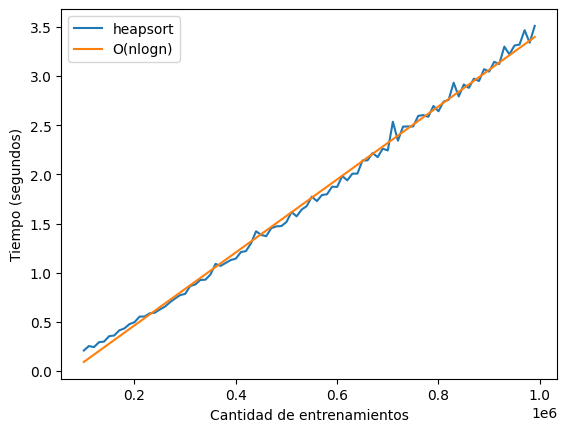
\includegraphics[width=1\textwidth]{img/tiempos.png}
\end{figure}

Como se puede apreciar, el algoritmo tiende a $\mathcal{O}\left(n \log n\right)$.

\section{Conclusiones}

Ac\'a ir\'ian las conclusiones de todo nuestro trabajo :)
}


\newpage
\end{document}